\subsection{What is Drools?}

JBoss Rules, or as it is more commonly known, Drools, is the leading opensource rules engine written in Java.
In this paper when we use the name "Drool" we are referring to the "Drools Expert" which is the rule engine module of the Drools Suite.
Drools started in 2001, but rose to prominence with it's 2005 2.0 release.  
It is an advanced inference engine using an enhanced version of the Rete algorithm, called Rete\-OO\cite{sottara2010configurable}, adapted to an object-oriented interface specifically for Java.
Designed to accept pluggable language implementations, it can also work with Python and .Net.
It is considered one of the most developed and supported rules platforms.

For rules to be executed there are 4 major components as demonstrated in figure \ref{fig:Drools_components}.
The production memory contains the rules.  
The rules are the focus of this thesis and therefore we will delve into much more detail later on these.
The working memory contains the facts.
The pattern matcher, using the aforementioned Rete\-OO algorithm will determine the possible rules to fire.
Rules that match will be placed on the agenda to be executed.
A conflict resolution strategy will decide which rule will fire.
If a rule specifies to halt or there are no matching rules left on the agenda, then the program extends.


\begin{figure}[h]
    \centering
    \fbox{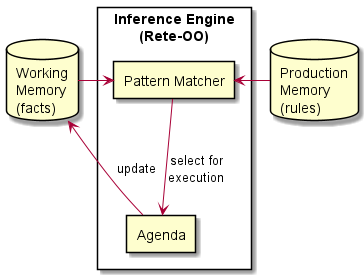
\includegraphics[width=0.95\textwidth]{Sections/images/components.png}}
    \caption{Drools components.}
    \label{fig:Drools_components}
\end{figure}


% WIP

% WIP END


\subsubsection{An explanatory example}
An example of a DRL file can be seen in listing \ref{listing:drl_file}. 

\begin{lstlisting}[language={[drl]Drools}, caption=Example Drools file., captionpos=b, label=listing:drl_file]
    package org.drools.examples.honestpolitician
 
    import org.drools.examples.honestpolitician.Politician;
    import org.drools.examples.honest politician.Hope;
     
    rule "We have an honest Politician"
        salience 10
        when
            exists( Politician( honest == true ) )
        then
            insertLogical( new Hope() );
    end
    
    rule "Hope Lives"
        salience 10
        when
            exists( Hope() )
        then
            System.out.println("Hurrah!!! Democracy Lives");
    end
    
    rule "Hope is Dead"
        when
            not( Hope() )
        then
            System.out.println( "We are all Doomed!!! Democracy is Dead" );
    end
    
    rule "Corrupt the Honest"
        when
            $p : Politician( honest == true )   
            exists( Hope() )
        then
            System.out.println( "I'm an evil corporation and I have corrupted " + $p.getName() );
            modify( $p ) { 
                setHonest( false ) 
            }
    end
\end{lstlisting}

Listing \ref{listing:drl_file} gives the Drools engine instructions on what actions to take when something changes in the working memory.
What this toy example does is reacts to when an honest politician is added to the working memory, prints a message celebrating the existence of said politician, corrupts her, gloats in a message and then prints a message of despair.
The code in listing \ref{listing:drl_file} does the following: 
\begin{enumerate}[topsep=2pt,itemsep=2pt,partopsep=2pt, parsep=2pt]
    \item on line 1 the package statement identifies the rule file
    \item on lines 3 and 4 the import statements describes which facts can be used
    \item the ``We have an honest Politician'' rule on line 6 does the following:
    \begin{enumerate}[topsep=2pt,itemsep=2pt,partopsep=2pt, parsep=2pt]
        \item using salience on line 7 it sets that this rule is to be run before rules with a lower salience
        \item on line 10 it checks the working memory for Politician facts with the honest property equal to true
        \item on line 12, if found then Hope facts will be inserted into the working memory
    \end{enumerate}
    \item the ``Hope Lives'' rule on line 15 does the following:
    \begin{enumerate}[topsep=2pt,itemsep=2pt,partopsep=2pt, parsep=2pt]
        \item line 18 check if any Hope facts exist
        \item on line 20, if found, it prints a message
    \end{enumerate}
    \item the ``Hope is Dead'' rule on line 23 does the following:
    \begin{enumerate}[topsep=2pt,itemsep=2pt,partopsep=2pt, parsep=2pt]
        \item checks if no Hope facts exist on line 25
        \item if none are found, on line 27, it prints a message 
    \end{enumerate}
    \item the ``Corrupt the Honest'' rule on line 30 does the following:
    \begin{enumerate}[topsep=2pt,itemsep=2pt,partopsep=2pt, parsep=2pt]
        \item line 32 checks for any Politician facts with the honest property equal to true, and sets them to the variable \$p
        \item line 33 checks if any Hope facts exist
        \item if both hope and politicians are found on line 35 it prints a message including the \$p variables name
        \item on line 36 to 38 it modifies the fact in working memory represented by \$p to change it's honest property 
    \end{enumerate}
\end{enumerate}